\documentclass[12pt, twoside]{article}
\usepackage[letterpaper, margin=1in, headsep=0.5in]{geometry}
\usepackage[english]{babel}
\usepackage[utf8]{inputenc}
\usepackage{amsmath}
\usepackage{amsfonts}
\usepackage{amssymb}
\usepackage{tikz}
\usetikzlibrary{quotes, angles}
\usepackage{graphicx}
\usepackage{enumitem}
\usepackage{multicol}
\usepackage{hyperref}

\newif\ifmeta
\metatrue %print standards and topics tags

\title{IB Mathematics}
\author{Chris Huson}
\date{September 2021}

\usepackage{fancyhdr}
\pagestyle{fancy}
\fancyhf{}
\renewcommand{\headrulewidth}{0pt} % disable the underline of the header
\raggedbottom


\fancyhead[LE]{\thepage}
\fancyhead[RO]{\thepage \\ Name: \hspace{4cm} \,\\}
\fancyhead[LO]{BECA / IB Math 03-Quadratic functions\\* 4 January 2022}

\begin{document}

\subsubsection*{3.2 Graphing quadratic functions}
%Equations of a straight line: $f(x)=mx+c$, $ax+by+d=0$, $(y-y_1)=m(x-x_1)$\\[0.25cm]
%Gradient: $\displaystyle m=\frac{y_2-y_1}{x_2-x_1}$\\[0.25cm]
Useful forms of equations for quadratics:\\[0.25cm] 
$f(x)=ax^2 + bx+c$, with $y$-intercept $c$, axis of symmetry $\displaystyle x=-\frac{b}{2a}$, zeros $\displaystyle x=\frac{-b \pm \sqrt{b^2-4ac}}{2a}$\\[0.25cm]
$g(x)=a(x-p)(x-q)$, with $x$-intercepts $p$, $q$ and axis of symmetry $\displaystyle x=\frac{p+q}{2}$\\[0.25cm] 
$h(x)=a(x-h)^2+k$, with vertex $(h,k)$
\vspace{1cm}
\begin{enumerate} 
\item Do Now: The function $f(x)=-x^{2}+6x-6$ is shown on the graph.
\begin{enumerate}
  \begin{multicols}{2}
      \item Write down its vertex as an ordered pair. \vspace{0.5cm}
      \item Write down the domain and range of $f$. \vspace{1cm}
      \item Draw on the graph the function \\$g(x)=-x+4$.
      \item Write down the two ordered pairs that satisfy both $f$ and $g$. \vspace{3cm}
      \begin{center}
      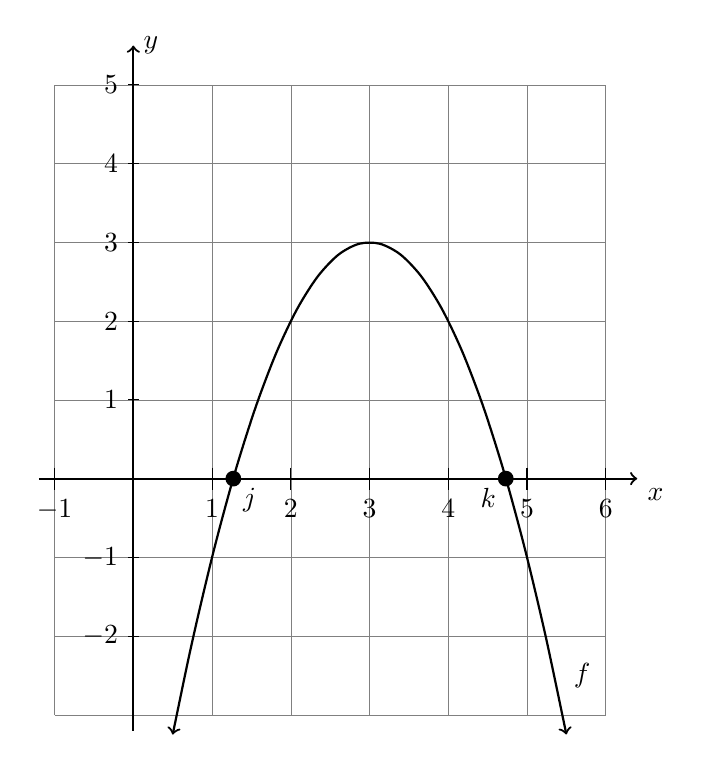
\begin{tikzpicture}[scale=1]
        \draw [help lines] (-1,-3) grid (6,5);
        \draw [thick, ->] (-1.2,0) -- (6.4,0) node [below right] {$x$};
        \draw [thick, ->] (0,-3.2)--(0,5.5) node [right] {$y$};
        \foreach \x in {-1, 1,2, ..., 6} \draw (\x cm,4pt) -- (\x cm,-4pt) node[anchor=north] {$\x$};
        \foreach \y in {-2,-1,1,2,..., 5} \draw (2pt,\y cm) -- (-2pt,\y cm) node[anchor=east] {$\y$};
        \fill (1.27,0) circle[radius=0.1] node[below right]{$j$};
        \fill (4.73,0) circle[radius=0.1] node[below left]{$k$};
        \draw [thick, <->,smooth,samples=20,domain=0.5:5.5] plot(\x,-\x*\x+6*\x-6);
        \node at (5.7,-2.5){$f$};
      \end{tikzpicture}
      \end{center}
    \end{multicols} 
    \vspace{0.5cm}
    \item Find the exact values of $j$ and $k$, the $x$-intercepts of $f$. (as an expression with radicals, not a decimal)
\end{enumerate} \vspace{3cm}

\newpage
\item Consider the function $f(x)=x^2+2x-3$.
    \begin{enumerate}
        \item Sketch the graph of $f$, for $-4 \leq x \leq 2$. Label the vertex and the intercepts.
        \item This function can also be written in the form $f(x)=(x-p)^2 -4$.\\* 
        Write down the value of $p$. \vspace{1.5cm}
        \item The graph of $f$ has two solutions for $f(x)=0$. Write down the solutions (or roots, zeros) of the function. \vspace{1.5cm}
        \item Hence, write down the function in factored form, $f(x)=(x-a)(x-b)$. \vspace{1.5cm}
    \end{enumerate}
    \begin{center}
    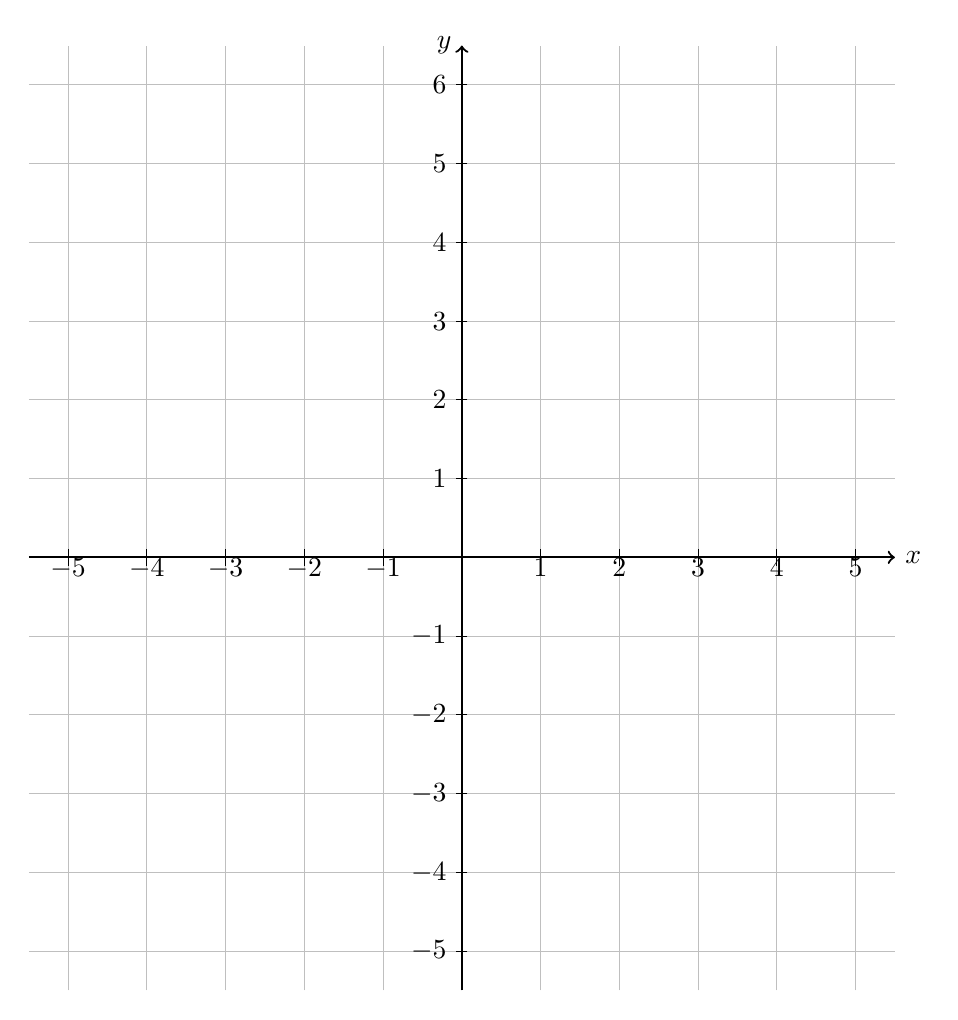
\begin{tikzpicture}
        \draw [thin, color=lightgray,, xstep=1.0cm,ystep=1.0cm] (-5.5,-5.5) grid (5.5,6.5);
        \foreach \x in {-5, -4, -3, -2, -1,1,2,3,4, 5}
        \draw[shift={(\x,0)},color=black] (0pt,-3pt) -- (0pt,3pt) node[below]  {$\x$};
        \foreach \y in {-5, -4, -3, -2, -1, 1,2,3,4, 5, 6}
        \draw[shift={(0,\y)},color=black] (2pt,0pt) -- (-2pt,0pt) node[left]  {$\y$};
        \draw [thick, ->] (-5.5,0) -- (+5.5,0) node [right] {$x$};
        \draw [thick, ->] (0,-5.5) -- (0,6.5) node [left] {$y$};
    \end{tikzpicture}
    \end{center}

\newpage
\subsection*{Sketching a quadratic function}
    \item   Given $f(x)=(x-3)^2-4$
    \begin{enumerate}[itemsep=0.9cm]
        \item Write down the vertex of the function as an ordered pair.
        \item Expand the function from vertex form to standard form, $ax^2+bx+c \text{ where } a, b, c \;  \epsilon \; \mathbb{R}$. \vspace{1cm}
        \item Write down the value of $f(0)$. Explain what this represents on the graph. \vspace{1cm}
        \item Factor the function. Write down the roots. \vspace{1cm}
        \item Sketch the function, labeling the intercepts with values and the vertex as an ordered pair. Show the axis of symmetry as a dotted line and label it with its equation.
        \begin{center}
            \begin{tikzpicture}
                \draw [thick, ->] (-4.5,0) -- (+4.5,0) node [right] {$x$};
                \draw [thick, ->] (0,-3.5) -- (0,4.5) node [left] {$y$};
            \end{tikzpicture}
            \end{center}
        \item Write down the domain and range of the function.
    \end{enumerate}

\newpage
  \item Let $f$ be a quadratic function. Part of the graph of $f$ is shown below.\\*
  The vertex is at $P(2,1)$ and the $y$-intercept is at $Q(0, 3)$.\\*

    \begin{figure}[!htbp]
    \begin{center}
    \begin{tikzpicture}
        \foreach \x in {-2, -1,1,2,3,4,5,6}
        \draw[shift={(\x,0)},color=black] (0pt,-3pt) -- (0pt,3pt) node[below]  {$\x$};

        \foreach \y in {-1,1,2,3,4,5,6}
        \draw[shift={(0,\y)},color=black] (2pt,0pt) -- (-2pt,0pt) node[left]  {$\y$};

        \draw [thick, ->] (-2.5,0) -- (+6.5,0) node [right] {$x$};
        \draw [thick, ->] (0,-1.5) -- (0,6.5) node [left] {$y$};

        \draw (2,1) circle[radius=2pt] node [below] {$P$};
        \fill (2,1) circle[radius=2pt];
        \draw (0,3) circle[radius=2pt] node [right] {$Q$};
        \fill (0,3) circle[radius=2pt];

        \draw [<->] plot[domain= -1:5] (\x, .5*\x*\x -2*\x +3);

    \end{tikzpicture}
    \end{center}
    \end{figure}

    \begin{enumerate}
        \item Write down the equation of the axis of symmetry.
        \item The function $f$ can be written in the form $f(x)=a(x-h)^2 +k$. \\*
        Write down the value of $h$ and of $k$.
        \item Find $a$.
    \end{enumerate}

\end{enumerate}
\end{document}